\textcolor{prime}{\textsf{Findings}} \\
\begin{itemize}
\item Using only first term of heuristic (Figure~\ref{fig:woheu}):
    \begin{itemize}
    \item the robot easily leaves a trot gait when disturbed
    \item departure from a trot gait reduces the stability of the system 
    \item the robot becomes unstable at higher amplitude disturbances
    \end{itemize}

\item Using both terms of the heuristic (Figure~\ref{fig:wheu}):
    \begin{itemize}
    \item $\mathrm{\sim50 \%}$ increase in maximum disturbance amplitude over a controller that only uses term 1
    \item $\mathrm{\sim100 \%}$ increase in maximum disturbance amplitude over the open loop response
    \item projecting $\vec{\omega}_0$ into nullspace forces the robot to utilize differing plunge and retract rates
    \item this helps maintain a trot gait
    \item system can still be forced to leave a trot gait if the disturbance is large enough
    \end{itemize}
\end{itemize}

\vspace{2EX}
\textcolor{prime}{\textsf{Future Work}} \\
\begin{itemize}
    \item We should test other possible heuristics for guiding the system back to a trot gait
	\item Test the controller on a real robot to verify its robustness given:
	\begin{itemize}
		\item motor dynamics
		\item waves produced by feet
		\item sensor noise
	\end{itemize}
\end{itemize}

\vspace{2EX}
\begin{figure}[h]
\centering
\begin{subfigure}[t]{0.47\textwidth}
    \centering
    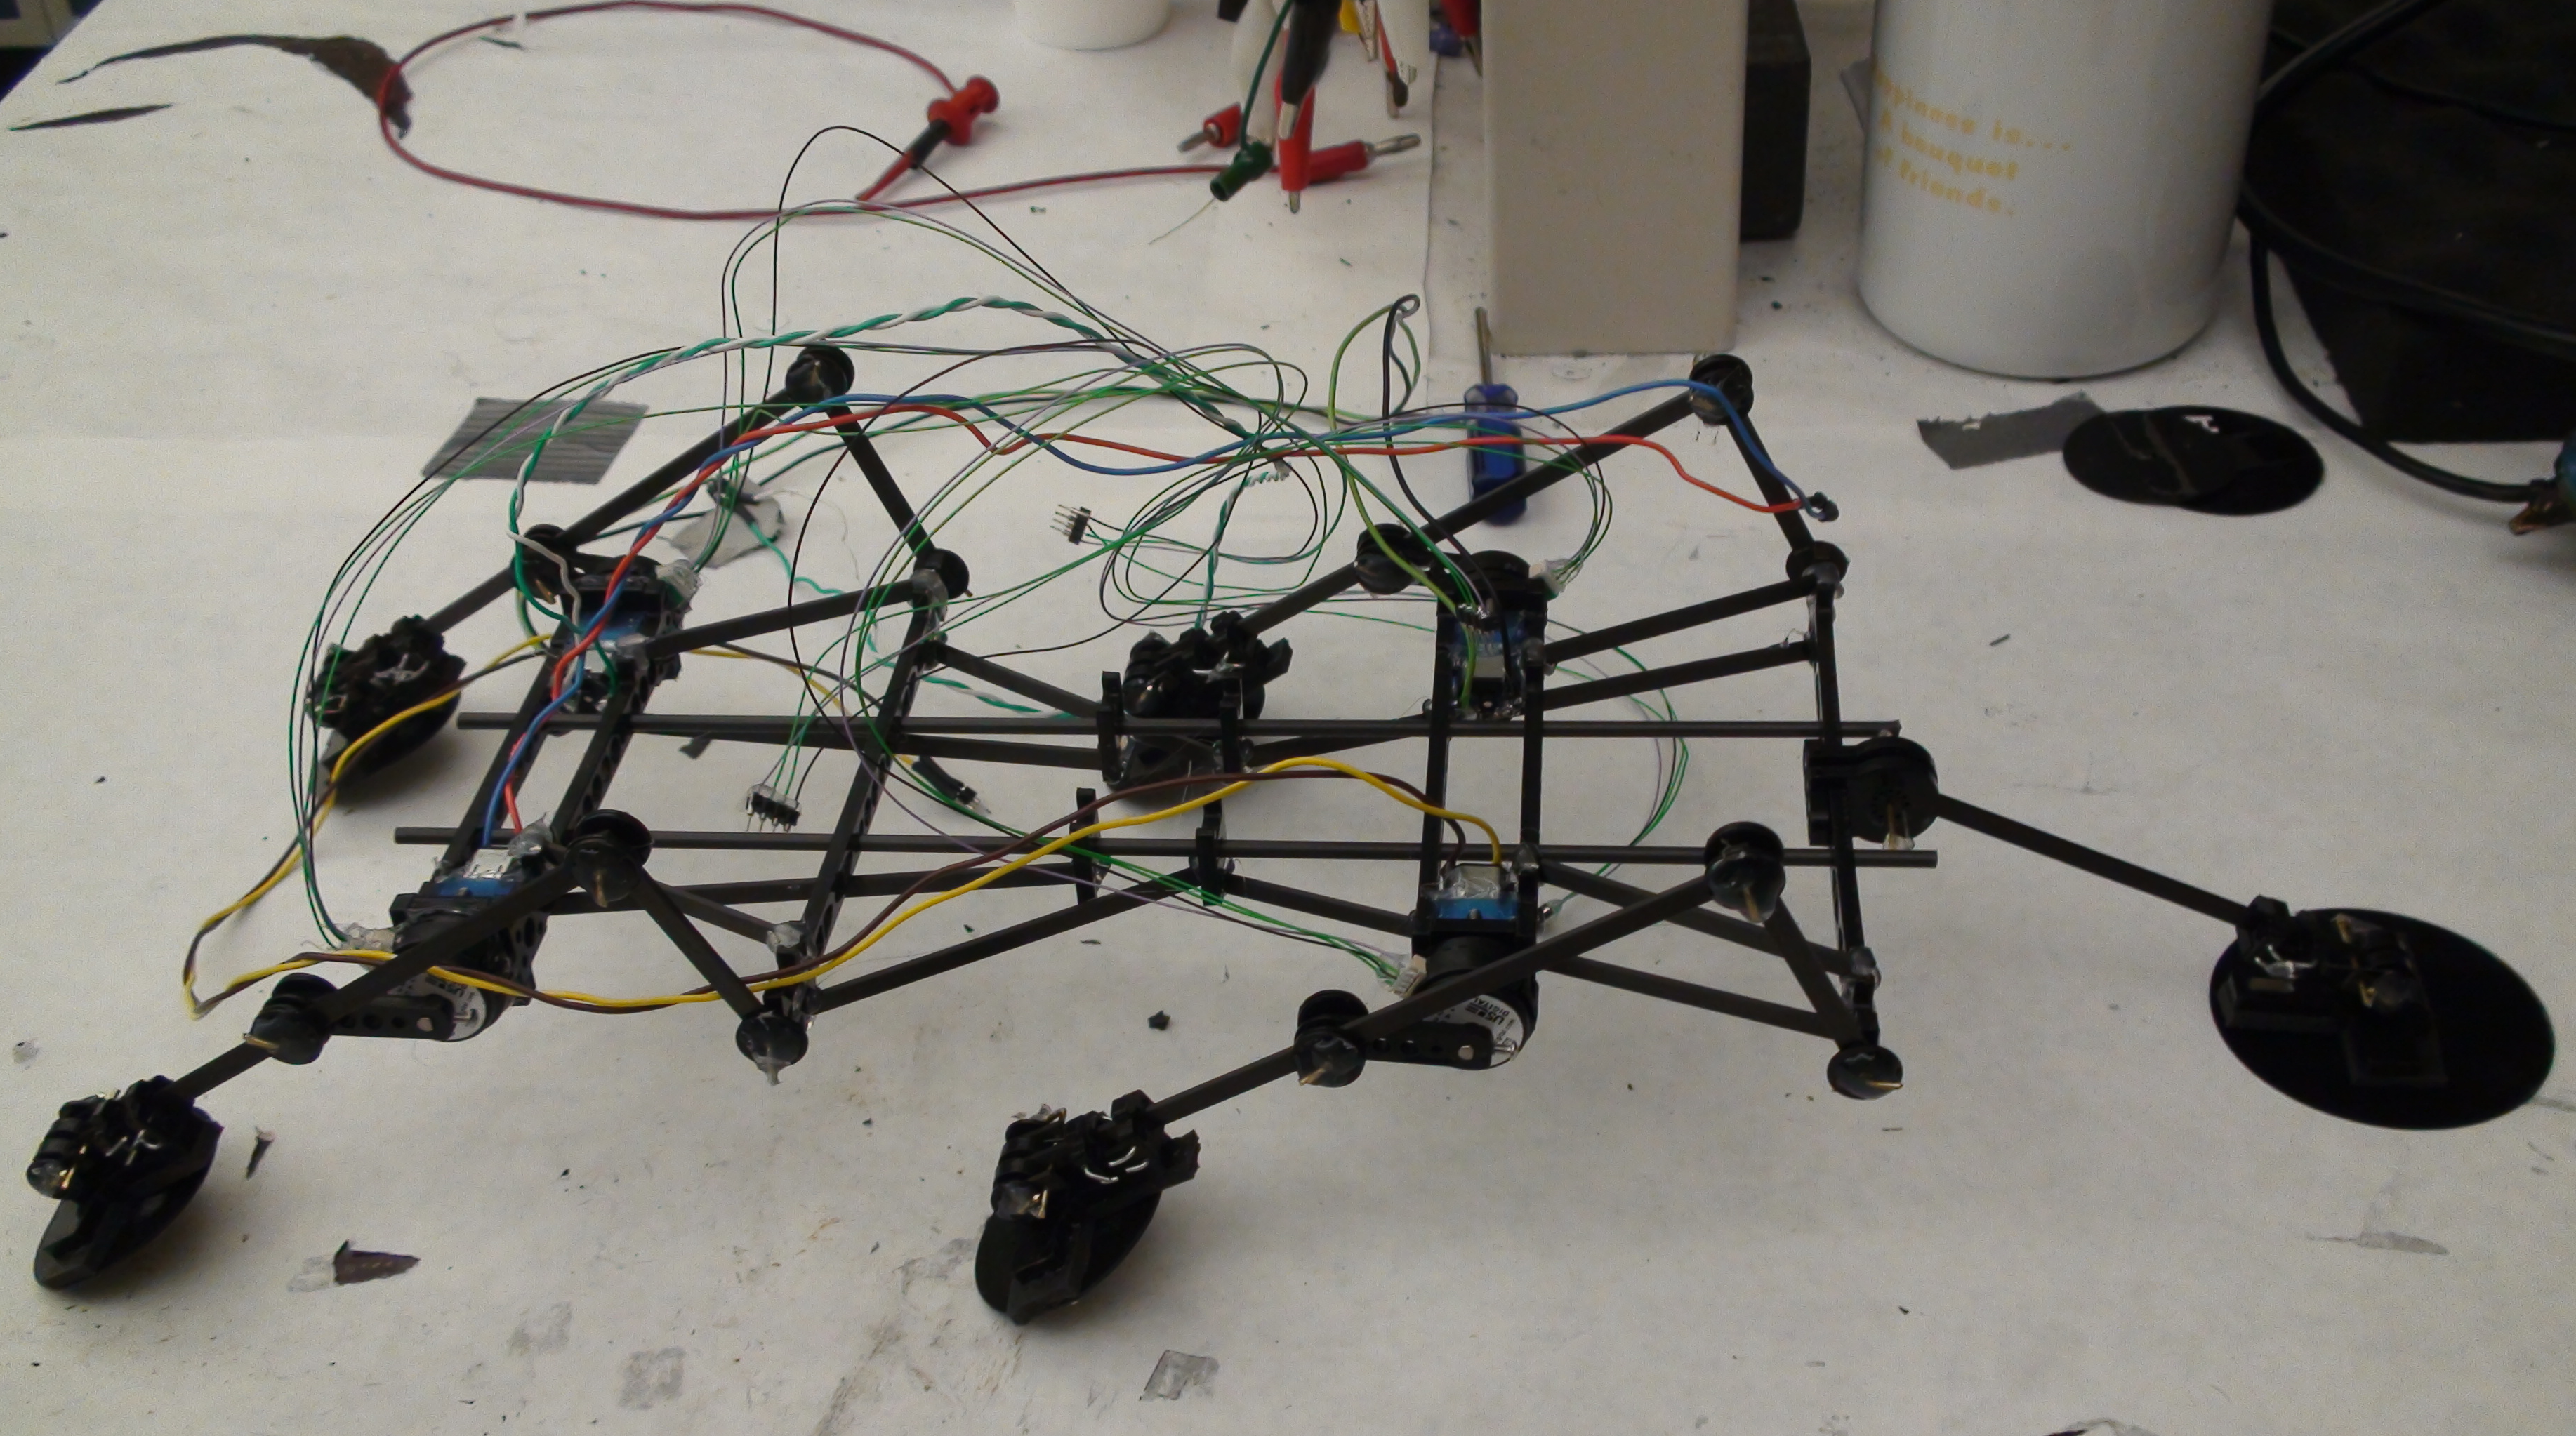
\includegraphics[height = 3.25in]{robot.JPG}
    \caption{Current Robot Hardware}
	\label{fig:robot}
\end{subfigure}
\quad
\begin{subfigure}[t]{0.47\textwidth}
    \centering
    \includegraphics[height = 3.25in]{basilisk-lizard.jpg}
    \caption{Real Basilisk Lizard}
	\label{fig:boom}
\end{subfigure}
\vspace{0.5EX}
\caption{The current robot design compared to a real Basilisk Lizard. A rotating boom setup will allow us to test the robot as it runs in a circle in a small pool.} 
\label{fig:test}
\end{figure}
\vspace{-.5in}
